\documentclass[letterpaper,12pt]{article}
\usepackage{tabularx} % extra features for tabular environment
\usepackage{amsmath}  % improve math presentation
\usepackage{float}
\usepackage{pdfpages}


\usepackage{graphicx} % takes care of graphic including machinery
\graphicspath{ {./figures/} }
%\usepackage[margin=1in,letterpaper]{geometry} % decreases margins
%\usepackage{cite} % takes care of citations
\usepackage[final]{hyperref} % adds hyper links inside the generated pdf file
\hypersetup{
	colorlinks=true,       % false: boxed links; true: colored links
	linkcolor=blue,        % color of internal links
	citecolor=blue,        % color of links to bibliography
	filecolor=magenta,     % color of file links
	urlcolor =blue         
}
\usepackage[margin = 1in,headsep=0.5cm,headheight=2cm,letterpaper]{geometry} 

\usepackage{fancyhdr}
\pagestyle{fancy}
\lhead{Student 1 : Ahmet Akman 2442366 \\ Student 2: Yusuf Toprak Yıldıran 2444149 \\ Assistant: Onur Selim Kılıç}
\rhead{Date: \today \\ Group: Wednesday Morning - 5} 
%\cfoot{center of the footer!}
\renewcommand{\headrulewidth}{0.1pt}
%

%\renewcommand{\footrulewidth}{0.4pt}



\begin{document}
\thispagestyle{empty}

\title{Spring 2022 EE214 Experiment 2  \protect\\ Miscellaneous Op-Amp Circuits}
\author{Ahmet Akman 2442366 \protect\\ Yusuf Toprak Yıldıran 2444149 \protect\\ Assistant: Onur Selim Kılıç}
\date{\today}
\maketitle
\tableofcontents
%\begin{abstract}
%abstract
%\end{abstract}
\section{Introduction}
In this experiment, miscellaneous op-amp circuits and three different setups of op-amp circuity are investigated. First, an independent current source circuit is set, and its behavior is required to be characterized. Then the clipper circuit is constructed, and the output is needed to be observed. Lastly, a negative resistance converter with two zener is built with two different setups. First, its i-v characteristics are expected to be observed; then, a square wave generator is expected to be set.
\section{Experimental Results and Discussion}
The results of the experiment are discussed in the following steps.
\subsection{Step 1}
In this step independent current source circuit given in Figure 1 is constructed. A potentiometer with 10K\(\Omega\) is connected to the one port as \(R_L\).
\begin{figure}[H]
    \centering
    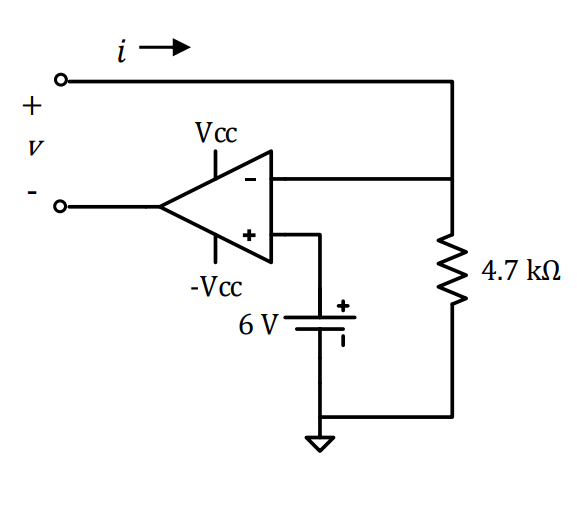
\includegraphics[width = 0.75\textwidth]{1SCH.png}
    \caption{Circuit schematic for the step 1}
\end{figure} 
To be able to obtain the maximum value of the resistance in which the one port still functions as an independent current source, the potentiometer is meticulously adjusted. So, the parameters given in Table 1 are obtained.
\begin{table}[H]
    \begin{center}
        \caption{Liner region boundary parameters}
        \vspace{2mm}
        \begin{tabular}{||c | c ||} 
            \hline
            The Current Value & Corresponding Resistance \\ [0.5ex] 
            \hline\hline
            1.24 mA & 8k\(\Omega\)    \\
            \hline
        \end{tabular}
    \end{center}
\end{table}

As a result, it can be concluded that the independent current source circuit functions as long as it is in the linear region; however when the op-amp saturates, it is no longer works. So, the circuit acts as an independent current source with 1.24mA until the load resistance is 8k\(\Omega\). 
\subsection{Step 2}
In this step, the clipper circuitry given in Figure 3 is constructed. \(V_{in}\) is set to \(3 sin (1000\pi t)\) from the signal generator.
\begin{figure}[H]
    \centering
    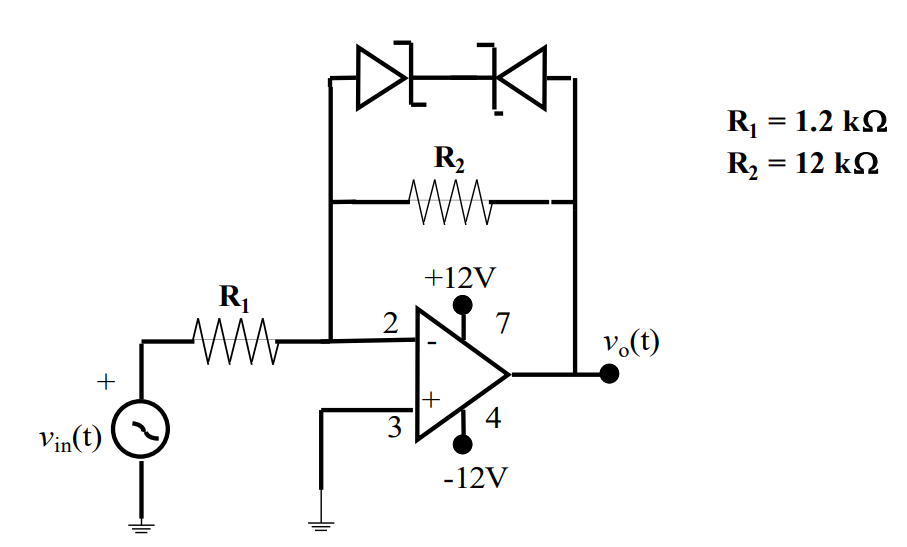
\includegraphics[width = 0.75\textwidth]{2SCH.png}
    \caption{Clipper circuit schematic for the step 2}
\end{figure} 
The plot given in Figure 4 is obtained as a result of \(V_o\) vs \(V_{in}\).
%TODO THE NAME OF THE PLOT FİLE BELOW SHOULD BE CHANGED
\begin{figure}[H]
    \centering
    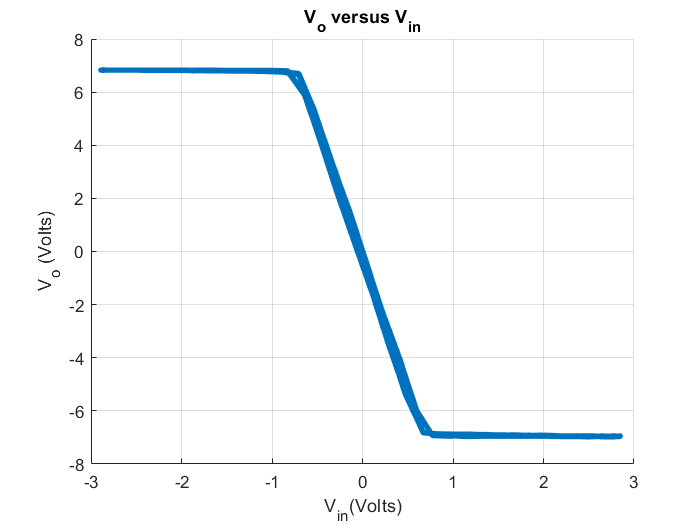
\includegraphics[width = 0.75\textwidth]{2.png}
    \caption{\(V_o\) vs \(V_{in}\)}
\end{figure} 
So it is observed that saturation voltages are not +12 and -12 Volts. This result is stemmed from the fact that in saturation regions, zener diodes are both open, but one from forwarding and another from the reverse. Which results in the sum of their forward opening voltage (\(\approx\)  1V ) and reverse-opening voltage ( \( \approx \) 6V ) to be 7 Volts. In the saturation region, they switch the forward-reverse and results in \( \approx\) 14V\(V_{pp}\)

\subsection{Step 3}

In this part, we set the negative resistance converter circuit given in Figure 4 below.
\begin{figure}[H]
    \centering
    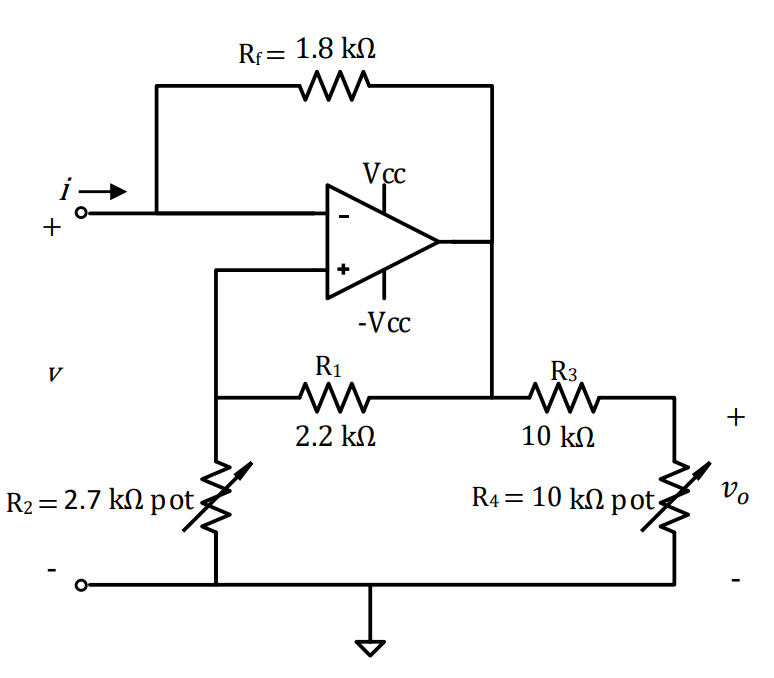
\includegraphics[width = 0.75\textwidth]{3SCH.png}
    \caption{Circuit schematic for the step 3}
\end{figure} 

  
\subsubsection{a)}
For this part a., we used 1.2k\(\Omega\) instead of the \(R_2\) 2.7k\(\Omega\) pot and adjusted the V as \(V(t) = 10sin(\pi t)V\) and obtained the i vs v characteristics by using DSO in X-Y mode in Figure 5. To obtain current i, we connected 1k\(\Omega\) resistor between common ground and non-inverting input port of the op-amp and measured the voltage across it, by doing this, we get the current in mA. Also, voltage v is obtained by measuring the input signal. From the oscilloscope, it can be seen that op-amp goes into + saturation or - saturation without being into linear region and the circuit is unstable.
%TODO THE NAME OF THE PLOT FİLE BELOW SHOULD BE CHANGED
\begin{figure}[H]
    \centering
    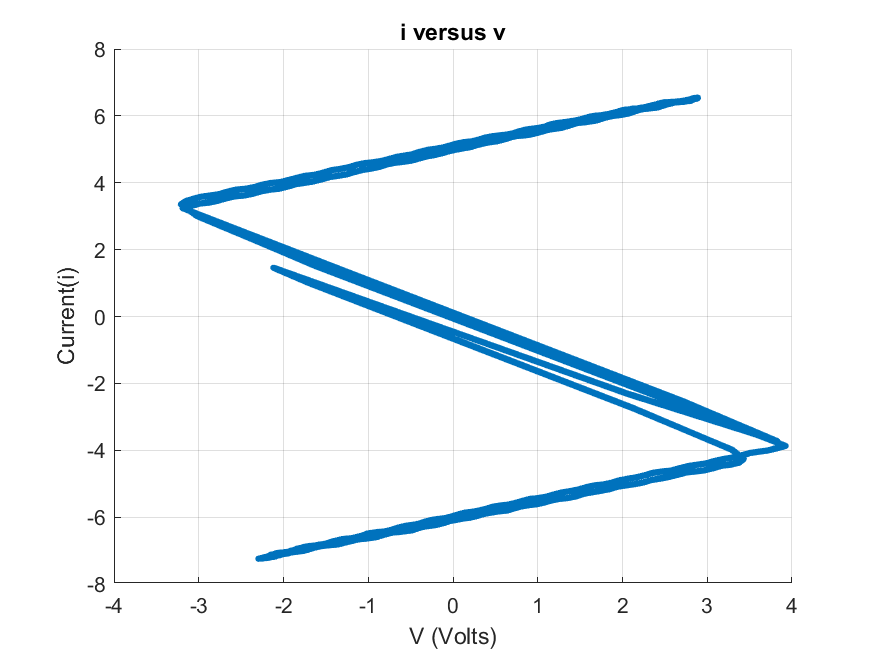
\includegraphics[width = 0.75\textwidth]{3a.png}
    \caption{\(i(t)\) vs \(V_{t}\)}
\end{figure} 


\subsubsection{b)}
In this subsection b. a 1\(\mu F\) capacitor is connected across the terminals between this one port circuit and \(R_2 \) and \(R_4 \) are adjusted until \(V_0(t)\) become a square wave of 2 volts peak-to-peak with the frequency of 500Hz. Then, \(R_2 \) and \(R_4 \) are recorded using a digital multimeter as a table which is given in the Table 2. It can be observed that experimental values are partially consistent with the preliminary work results given in Table 3. Also time constant \(\tau\) is found by multiplying \(R_f\) with the capacitance of the capacitor given in Table 2. 
\begin{table}[H]
    \begin{center}
        \caption{Experimental Results of \(R_2\),\(R_4\) and \(\tau \).}
        \vspace{2mm}
        \begin{tabular}{||c | c | c ||} 
            \hline
            \(R_2\) & \(R_4\) &  \(\tau \) \\ [0.5ex] 
            \hline\hline
            0.46k\(\Omega\) & 2.4k\(\Omega\) &  1.8x\(10^-6\)s \\
            \hline
        \end{tabular}
    \end{center}
\end{table}

\begin{table}[H]
    \begin{center}
        \caption{Preliminary Work Results of \(R_2\) and \(R_4\).}
        \vspace{2mm}
        \begin{tabular}{||c | c ||} 
            \hline
            \(R_2\) & \(R_4\) \\ [0.5ex] 
            \hline\hline
            1.63k\(\Omega\) & 2k\(\Omega\)   \\
            \hline
        \end{tabular}
    \end{center}
\end{table}


Then, \(V_C(t)\) and \(V_0(t)\) are observed on the DSO screen as seen in Figure 6.
From this part b. it can be said that an adjustable square wave signal can be obtained without applying an input signal to a negative resistance converter and the frequency of this signal can be adjusted by changing the potentiometer \(R_2\) and the amplitude can be adjusted by changing the \(R_4\).
%TODO THE NAME OF THE PLOT FİLE BELOW SHOULD BE CHANGED
\begin{figure}[H]
    \centering
    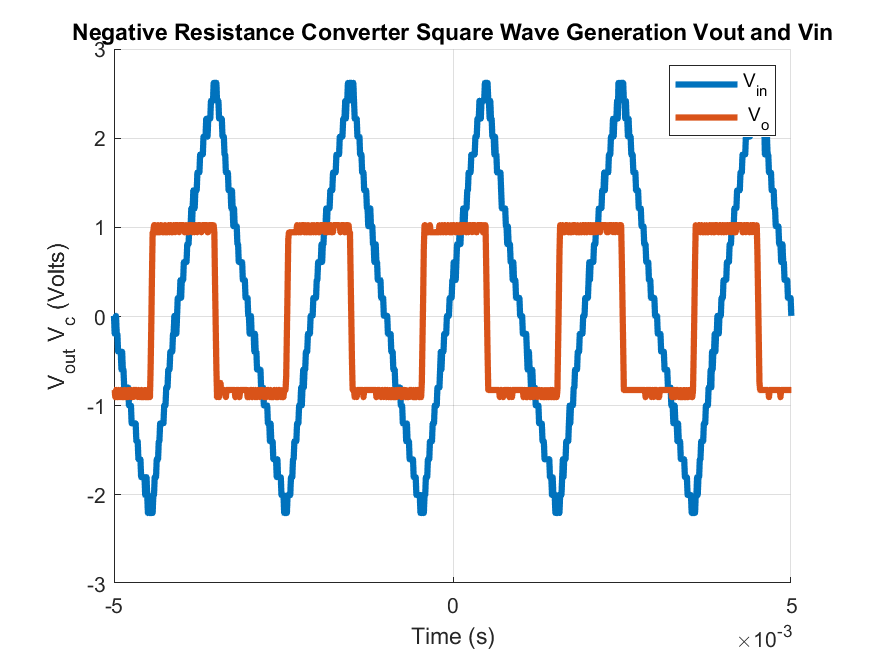
\includegraphics[width = 0.75\textwidth]{3b.png}
    \caption{\(V_C(t)\)  \(V_0(t)\) vs Time}
\end{figure} 


\section{Conclusion}
In this experiment, miscellaneous op-amp circuits have experimented with three different op-amp setups: independent current source, clipper, and negative resistance converter. First, it is observed where the independent current source works and the maximum load resistance obtained. Then it is observed that the behavior of the clipper circuit explained the reason why saturation regions are different. Lastly, a negative resistance circuit is constructed. Its one port i-v characteristics are obtained, then a square wave generator is configured with the same setup with the help of a capacitor. The target frequency and amplitude values are achieved, and the variables are noted. To sum up, in this experiment, three different setups of the op-amp are investigated.
\section*{Appendix A}
\begin{itemize}
    \item PreLab Preparation 4 hours
    \item Experimental Work 2  hours
    \item Report Writing 4 hours
\end{itemize}

\end{document}

%%%%%%%%%%%%%%%%%%%%%%   EXAMPLE TABLE   %%%%%%%%%%%%%%%%%%%%%%%%%%%%%%%%
\begin{table}[H]
\begin{center}
    \caption{Resistance reading by color code convention.}
    \vspace{2mm}
    \begin{tabular}{||c | c | c||} 
        \hline
        Color Order & Value & Tolerance \\ [0.5ex] 
        \hline\hline
        Brown / Black / Red / Gold & 1k\( \Omega \) & \( \% \) 5  \\ 
        \hline
        Yellow / Violet / Red / Gold & 4.7k\( \Omega \) & \( \% \) 5   \\
        \hline
        Brown / Grey / Orange / Gold & 18k\( \Omega \) & \( \% \) 5  \\ [1ex] 
        \hline
    \end{tabular}
\end{center}
\end{table}


%%%%%%%%%%%%%%%%%%%%%%   EXAMPLE IMAGE   %%%%%%%%%%%%%%%%%%%%%%%%%%%%%%%%
\begin{figure}[H]
\centering
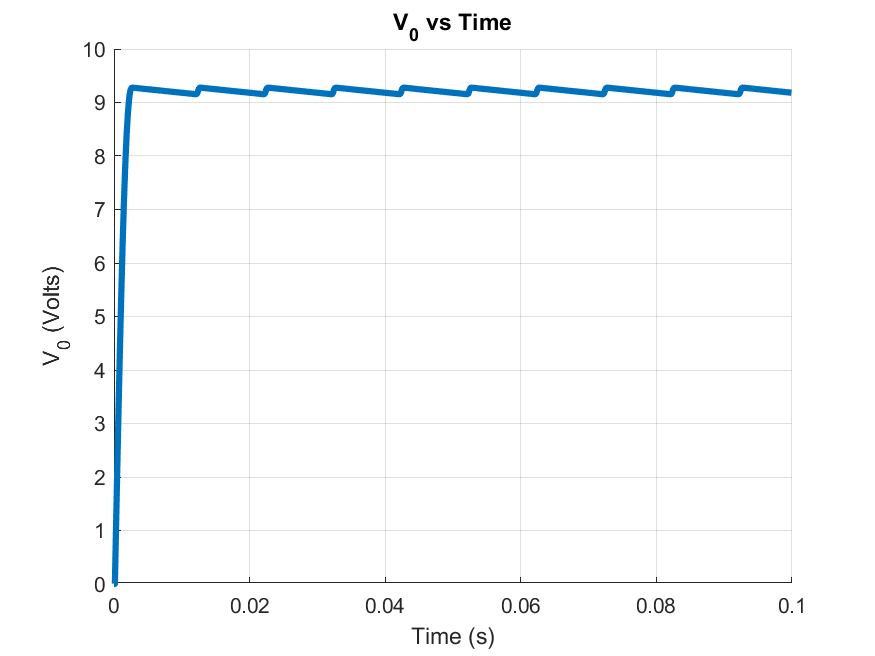
\includegraphics[width = 0.75\textwidth]{5.png}
\caption{Circuit schematic for the step 5}
\end{figure} 

%%%%%%%%%%%%%%%%%%%%%%   EXAMPLE IMAGE FROM PDF   %%%%%%%%%%%%%%%%%%%%%%%%%%%%%%%%
\begin{figure}[H] \centering{
	\includegraphics[scale=0.25]{2a_plot.pdf}}
	\caption{Experiment 2}
\end{figure}
	